\begin{Problem}
	Die Differentialgleichung für den harmonischen Oszillator in zwei Dimensionen lautet:
	\[
		\ddot{\va x}(t)+\omega^2\va x=0\qquad\text{mit }\omega=\sqrt{\frac{k}{m}} 
	.\] 
Entwickeln Sie den Ortsvektor $x(t)$ und seine zeitlichen Ableitungen in der Polarkoordinatenbasis $\{\vu e_r , \vu e_\phi \}$ und überzeugen Sie sich, dass die so aus (1) folgenden Differentialgleichungen den Bewegungsgleichungen entsprechen, die Sie wie in der Vorlesung mittels der Euler-Lagrange-Gleichung
\[
	\left( \dv{t}\pdv{\dot{q_i}}-\pdv{q_i} \right) L(q(t),\dot{q}(t),t)=0
\] 
direkt aus der Lagrangefunktion in Polarkoordinaten $q_i=r,\phi$ erhalten.
\end{Problem}
\begin{proof}
	\begin{align*}
		\va x=&\begin{pmatrix} r\cos\phi \\ r\sin\phi \end{pmatrix} \\
		\dot{\va x}=&\dot{r}\begin{pmatrix} \cos\phi\\ \sin\phi \end{pmatrix} +r\dot\phi \begin{pmatrix} -\sin\phi \\ \cos\phi \end{pmatrix} \\ 
		\ddot{\va x}=&\ddot{r}\begin{pmatrix} \cos\phi \\ \sin\phi \end{pmatrix} +(2\dot{r}\dot{\phi}+r\ddot{\phi})\begin{pmatrix} -\sin\phi \\ \cos\phi \end{pmatrix}+r\dot{\phi}^2 \begin{pmatrix} -\cos\phi \\ -\sin\phi \end{pmatrix} \\
		=&(\ddot{r}-r\dot{\phi}^2)\begin{pmatrix} \cos\phi \\ \sin \phi \end{pmatrix} +\left( 2\dot{r}\dot{\phi}+r\ddot{\phi} \right) \begin{pmatrix} -\sin\phi \\ \cos\phi \end{pmatrix} 
	\end{align*}
	Weil $(\cos\phi, \sin\phi)^T$ und $(\sin\phi, \cos\phi)^T$ linear unabhängig (sogar orthogonal) sind, kann die Gleichung $\ddot{\va x}+\omega^2\va x(t)$ als
	\begin{align*}
		\ddot{r}-r\dot{\phi}^2+\omega^2 r=&0\\
		2\dot{r}\dot{\phi}+r\ddot{\phi}=&0
	\end{align*}
	Man schreibt auch direkt die Lagrangefunktion:
	\[
		L=\frac{1}{2}m\left( \dot{r}^2+r^2\dot{\phi}^2 \right)-\frac{1}{2}m\omega^2r^2 
	.\] 
	Die Euler-Lagrange-Gleichungen sind
	\begin{align*}
		r:& m\ddot{r}-mr\dot{\phi}^2+m\omega^2r=0\\
		  & \ddot{r}-r\dot{\phi}^2+\omega^2 r=0\\
		\phi:& \dv{t}\left( r^2\dot{\phi} \right) =0\\
		     & 2r\dot{r}\dot{\phi}+r^2\ddot{\phi}=0\\
		     & 2\dot{r}\dot{\phi}+r\ddot{\phi}=0.\qedhere
	\end{align*}
\end{proof}
\begin{Problem}
	Eine Punktmasse $m$ rotiere reibungslos auf einer Tischplatte. Über einen gespannten Faden der Länge $l$ $(l = r + s)$ sei sie durch ein Loch in der Platte mit einer anderen Masse $M$ verbunden (s. Skizze). Wie bewegt sich $M$ unter dem Einfluss der Schwerkraft?
	\begin{enumerate}
		\item Formulieren Sie die Zwangsbedingungen.
		\item Stellen Sie die Lagrange-Funktion in den generalisierten Koordinaten $s$ und $\varphi$ auf und ermitteln Sie daraus die Bewegungsgleichungen. Zeigen Sie, dass $\pdv{L}{\dot{\varphi}}  = \text{const} \equiv C$ gilt.
		\item Verwenden Sie das Ergebnis aus Teilaufgabe 2, um die $\varphi$-Abhängigkeit in der Differentialgleichung für $s$ zu eliminieren. Betrachten Sie nun den Gleichgewichtsfall $s(t) = \text{const}$ und finden Sie einen Ausdruck für die resultierende Rotationsgeschwindigkeit $\dot{\varphi}(t) = \text{const} \equiv \omega_0$ der Masse m. Ausgehend vom Gleichgewichtsfall, unter welchen Bedingungen rutscht die Masse $M$ nach oben, wann nach unten?
		\item Diskutieren Sie das Ergebnis für die Anfangsbedingung $\dot{\varphi}(t_0) = 0$.
	\end{enumerate}
\end{Problem}
\begin{proof}
	\begin{enumerate}
		\item $\dv{l}{t}=0$.
		\item \[
				L=\frac{1}{2}m\left( \dot{r}^2+r^2\dot{\varphi}^2 \right) +Mg(l-r)
		.\] 
		Weil $\pdv{L}{\varphi}=0$, gilt aus der Euler-Lagrange-Gleichungen $\dv{t}\pdv{L}{\dot{\varphi}}=0$, also $\pdv{L}{\dot{\varphi}}=\text{const}\equiv C$.
	\item Weil $\pdv{L}{\dot{\varphi}}=mr^2\dot{\varphi}\equiv C$, gilt
	\end{enumerate}
\end{proof}
\begin{Problem}
	Eine einmal gefaltete Schnur mit Gesamtl\"{a}nge $l$ und konstanter Masse pro L\"{a}nge $\rho$ bewegt sich auf der $x$-Achse. Die Endpunkte der Schnur seien mit $x_1(t)$ und $x_2(t)$ bezeichnet. Die Stelle, an der die Schnur gefaltet ist, sei mit $y(t)$ bezeichnet.
	\begin{center}
		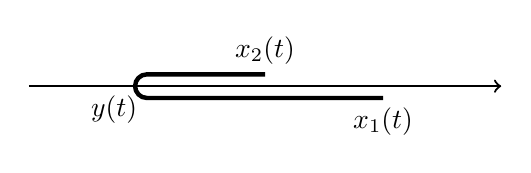
\begin{tikzpicture}[scale=3]
			\draw[thick, ->] (0.5,0) -- (2.5,0);
			\draw[ultra thick] (2,-0.05) -- ++(-1,0) arc(270:90:0.05) -- ++(0.5,0);
			\draw (1,-0) node[anchor=north east] {$y(t)$};
			\draw (1.5,0.05) node[anchor=south] {$x_2(t)$};
			\draw (2,-0.05) node[anchor=north] {$x_1(t)$};
		\end{tikzpicture}
	\end{center}
	\begin{enumerate}
		\item Geben Sie die Zwangsbedingungen des Systems an.
		\item Geben Sie eine Langrangefunktion des Systems an.

			{\footnotesize{Betrachten Sie f\"{u}r die kinetische Energie T die Endpunkte $x_1$ und $x_2$, deren ``Masse" durch die integrierte Masse des Schnurst\"{u}cks zwischen $x_1$ und $y$ bzw. $x_2$ und $y$ gegeben ist.}}
\item Die Lagrangefunktion kann in den Relativ- und Schwerpunktskoordinaten
	\[
		\xi=x_1-x_2\text{ und }X=\frac{1}{2l}\left[ (x_1-y)(x_1+y)+(x_2-y)(x_2+y) \right] 
	\]
	zu
	\[
		L=\frac{M}{2}\dot{X}^2+\frac{\mu}{2}\dot{\xi}^2
	\]
umgeschrieben werden, wobei $M$ und $\mu$ Funktionen von $X$ und $\xi$ sind. Bestimmen Sie $M$ und $\mu$ durch den Vergleich der Lagrangefunktionen in Koordinaten $(x_1, x_2)$ und $(X, \xi)$.
	\end{enumerate}
\end{Problem}
\begin{proof}
	\begin{enumerate}
\item $l=x_2(t)-y(t)+x_1(t)-y(t)=x_1(t)+x_2(t)-2y(t)$
\end{enumerate}
\end{proof}
